\documentclass[12pt]{article}
\usepackage[pdftex]{color, graphicx}
\usepackage{amsmath, amsfonts, amssymb, mathrsfs}
\usepackage{dcolumn}
\usepackage{natbib}
\usepackage{graphicx}
\usepackage{geometry}
\usepackage{listings}


\title{Mid2 Report}
\author{LI XU}
%\date{Dec.2 2015}

\geometry{left=2cm,right=2cm,top=1.5cm,bottom=1.5cm}
\begin{document}
\maketitle

\section{Modifications}
Similar to the cifar10\_cnn example. I use image\_data\_generator function to enable the image random shifting and rotating when training. Also I set the epochs to $5$. The model fit code is below:
\begin{lstlisting}[language=R,breaklines=true]
datagen = image_data_generator(rotation_range=8, 
width_shift_range=0.08, 
shear_range=0.3,
height_shift_range=0.08, 
zoom_range=0.08)
datagen %>% fit_image_data_generator(x_train)
model %>% fit_generator(
flow_images_from_data(x_train, y_train, datagen, batch_size = batch_size),
steps_per_epoch = as.integer(60000/64), 
epochs = 5, 
validation_data = list(x_test, y_test),
validation_steps=10000/64
)
\end{lstlisting}


\section{Results}
\begin{lstlisting}[language=R,breaklines=true]
Epoch 1/5
937/937 [==============================] - 19s 20ms/step - loss: 0.0599 - acc: 0.9832 - val_loss: 0.0267 - val_acc: 0.9927
Epoch 2/5
937/937 [==============================] - 19s 20ms/step - loss: 0.0609 - acc: 0.9830 - val_loss: 0.0185 - val_acc: 0.9948
Epoch 3/5
937/937 [==============================] - 19s 20ms/step - loss: 0.0595 - acc: 0.9832 - val_loss: 0.0208 - val_acc: 0.9934
Epoch 4/5
937/937 [==============================] - 19s 20ms/step - loss: 0.0589 - acc: 0.9836 - val_loss: 0.0186 - val_acc: 0.9948
Epoch 5/5
937/937 [==============================] - 19s 20ms/step - loss: 0.0600 - acc: 0.9835 - val_loss: 0.0188 - val_acc: 0.9947
> scores <- model %>% evaluate(
+   x_test, y_test, verbose = 0
+ )
> cat('Test loss:', scores[[1]], '\n')
Test loss: 0.0187528 
> cat('Test accuracy:', scores[[2]], '\n')
Test accuracy: 0.9947 
\end{lstlisting}
The figure during training is in Figure (1). The testing accuracy is $99.47\%$
\begin{figure}
	\centering
	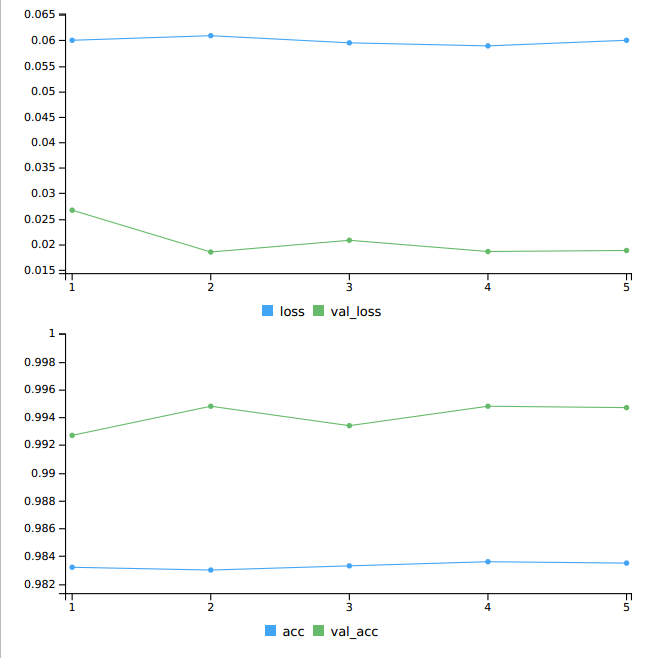
\includegraphics[scale=1]{lines.png}
	\caption{Results plot.}
\end{figure}

\clearpage
\appendix
\section{R code}
\begin{lstlisting}[language=R]
library(keras)

# Data Preparation -----------------------------------------------------

batch_size <- 128
num_classes <- 10
epochs <- 12

# Input image dimensions
img_rows <- 28
img_cols <- 28

# The data, shuffled and split between train and test sets
mnist <- dataset_mnist()
x_train <- mnist$train$x
y_train <- mnist$train$y
x_test <- mnist$test$x
y_test <- mnist$test$y

# Redefine  dimension of train/test inputs
x_train <- array_reshape(x_train, c(nrow(x_train), img_rows, img_cols, 1))
x_test <- array_reshape(x_test, c(nrow(x_test), img_rows, img_cols, 1))
input_shape <- c(img_rows, img_cols, 1)

# Transform RGB values into [0,1] range
x_train <- x_train / 255
x_test <- x_test / 255

cat('x_train_shape:', dim(x_train), '\n')
cat(nrow(x_train), 'train samples\n')
cat(nrow(x_test), 'test samples\n')

# Convert class vectors to binary class matrices
y_train <- to_categorical(y_train, num_classes)
y_test <- to_categorical(y_test, num_classes)

# Define Model -----------------------------------------------------------

# Define model
model <- keras_model_sequential() %>%
layer_conv_2d(filters = 32, kernel_size = c(3,3), activation = 'relu',
input_shape = input_shape) %>% 
layer_conv_2d(filters = 64, kernel_size = c(3,3), activation = 'relu') %>% 
layer_max_pooling_2d(pool_size = c(2, 2)) %>% 
layer_dropout(rate = 0.25) %>% 
layer_flatten() %>% 
layer_dense(units = 128, activation = 'relu') %>% 
layer_dropout(rate = 0.5) %>% 
layer_dense(units = num_classes, activation = 'softmax')
model %>% compile(
loss = loss_categorical_crossentropy,
optimizer = optimizer_adadelta(),
metrics = c('accuracy')
)


datagen = image_data_generator(rotation_range=8, 
width_shift_range=0.08, 
shear_range=0.3,
height_shift_range=0.08, 
zoom_range=0.08)
datagen %>% fit_image_data_generator(x_train)
model %>% fit_generator(
flow_images_from_data(x_train, y_train, datagen, batch_size = batch_size),
steps_per_epoch = as.integer(60000/64), 
epochs = 5, 
validation_data = list(x_test, y_test),
validation_steps=10000/64
)

scores <- model %>% evaluate(
x_test, y_test, verbose = 0
)

# Output metrics
cat('Test loss:', scores[[1]], '\n')
cat('Test accuracy:', scores[[2]], '\n')

\end{lstlisting}
\end{document}